\documentclass{article}

% Language setting
% Replace `english' with e.g. `spanish' to change the document language
\usepackage[english]{babel}
\usepackage{}
\usepackage{listings}


% Set page size and margins
% Replace `letterpaper' with `a4paper' for UK/EU standard size
\usepackage[letterpaper,top=2cm,bottom=2cm,left=3cm,right=3cm,marginparwidth=1.75cm]{geometry}

% Useful packages
\usepackage{amsmath}
\usepackage{graphicx}
\usepackage[colorlinks=true, allcolors=blue]{hyperref}


\title{Percolation}
\author{Cheng, Jui-Hung}

\begin{document}
\maketitle

\section{Introduction}

~~~~Percolation theory describe the phenomenon when random links or lattice are added to a network or a graph. It is about whether some nodes will be  connected, disconnected, or merge into a bigger cluster.

A representative question is as follow. Assume that, there is a material with several holes. Will the liquid be able to reach the bottom if we pour it from the top? The above question can be modelled into the following mathematical question. 

Constructing a n*n*n 3-dimensional Vertex Network. The lattices between each two neighbors will be connected with probability p, and unconnected with 1-p and what is the probability p when there is a path that go from the top to the bottom. The above question is now called bond-percolation. There is another question called site-percolation.

\subsection{Model explanation}

~~~~The model I research is a n*n two-dimensional Vertex Network bond-percolation. The lattices between two neighbor Vertex will be connected with probability P that is called bond. Analyze the clusters in the network when the probability is p.

\section{Percolation implementation}

To implement percolation, I separate the code into five parts.
\begin{enumerate}
    \item Network Construction 
    \item Percolation function
    \item DFS travel
    \item printing cluster information 
\end{enumerate}

\subsection{Network Construction}
~~~~To implement the model, we will need a Vertex Network to store the information of the bond. I use a class named Node represent all the possible lattice. That is each Node will have up, down, left right four nodes that can connect to the neighbor nodes and the information that check if the node is connected or not.

\begin{figure}[h]
\centering
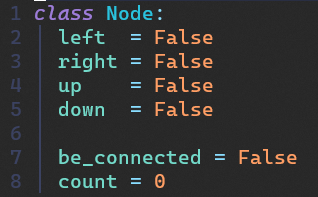
\includegraphics[width=0.28\linewidth]{Node.png}
\caption{\label{fig:Node}Each node connect to the four direction neighbor nodes}
\end{figure}


\subsection{Percolation function}
~~~~Traveling the whole map and decide whether connecting each lattice between neighbor nodes with the random function and update the information in both neighbor nodes after adding lattice.

\begin{figure}[h]
\centering
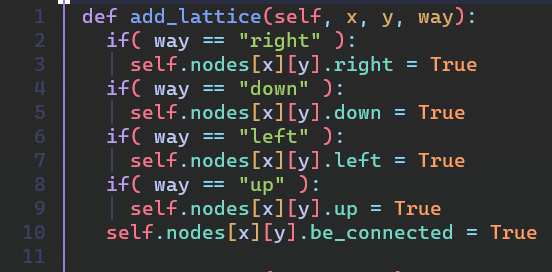
\includegraphics[width=0.55\linewidth]{add_latice.png}
\caption{\label{fig:add_lattice} adding the lattice in one direction but update information in both nodes}
\end{figure}

However,  the lattice in the Vertex Network is bi-directional, that is, we just have to add lattice in down and right direction.

\subsection{DFS travel}

~~~~Using Depth First Search Traveling to count the nodes connected in each cluster. Then DFS traveling the cluster again to label the cluster and add the information to the nodes in the cluster.

\begin{figure}[h]
\centering
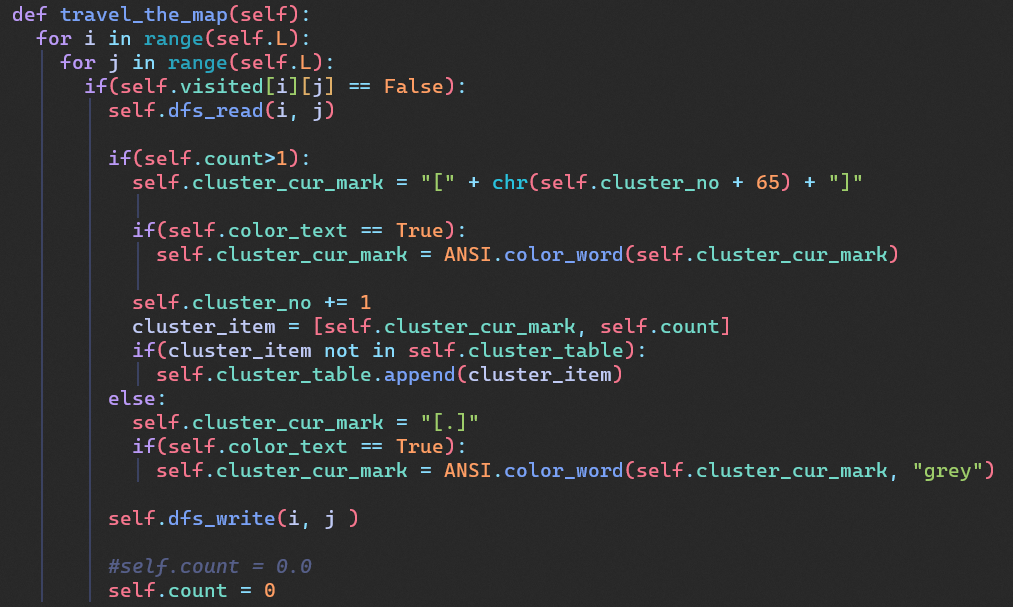
\includegraphics[width=0.6\linewidth]{DFS traveling.png}
\caption{\label{fig:DFS}DFS traveling two times for counting number in cluster, and adding information in cluster}
\end{figure}

\subsection{Printing cluster information}
~~~~Collecting the information of cluster when traveling the map, and print the cluster label information, such as : the cluster A connected two nodes, and cluster B connected 20 nodes.

\subsection{ANSI color}
~~~~Using the plain text to print the map is hard to analyzing the cluster distribution, therefore, I import the ANSI\_color library to display the map and cluster information with color. 

\newpage

\begin{figure}[h]
\centering
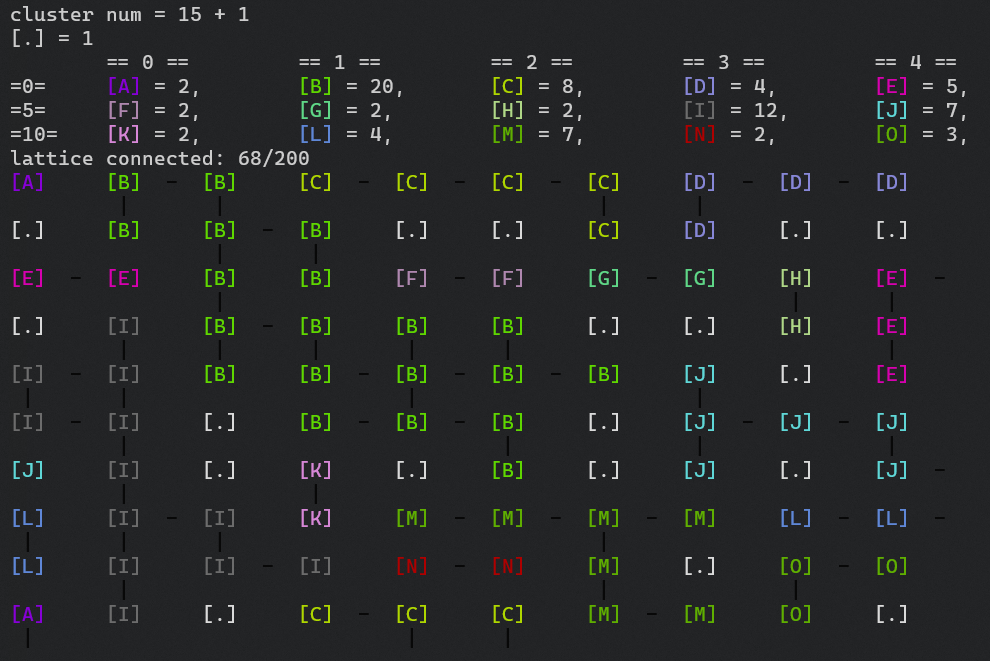
\includegraphics[width=0.45\linewidth]{Percolation result.png}
\caption{\label{fig:DFS}DFS traveling two times for counting number in cluster, and adding information in cluster}
\end{figure}

\section{Analyzing}

when the prob is under 0.45, there are at least 25 clusters in a map, and most of the clusters connected at most 50 nodes. 


\begin{figure}[h]
   \begin{minipage}{0.48\textwidth}
     \centering
     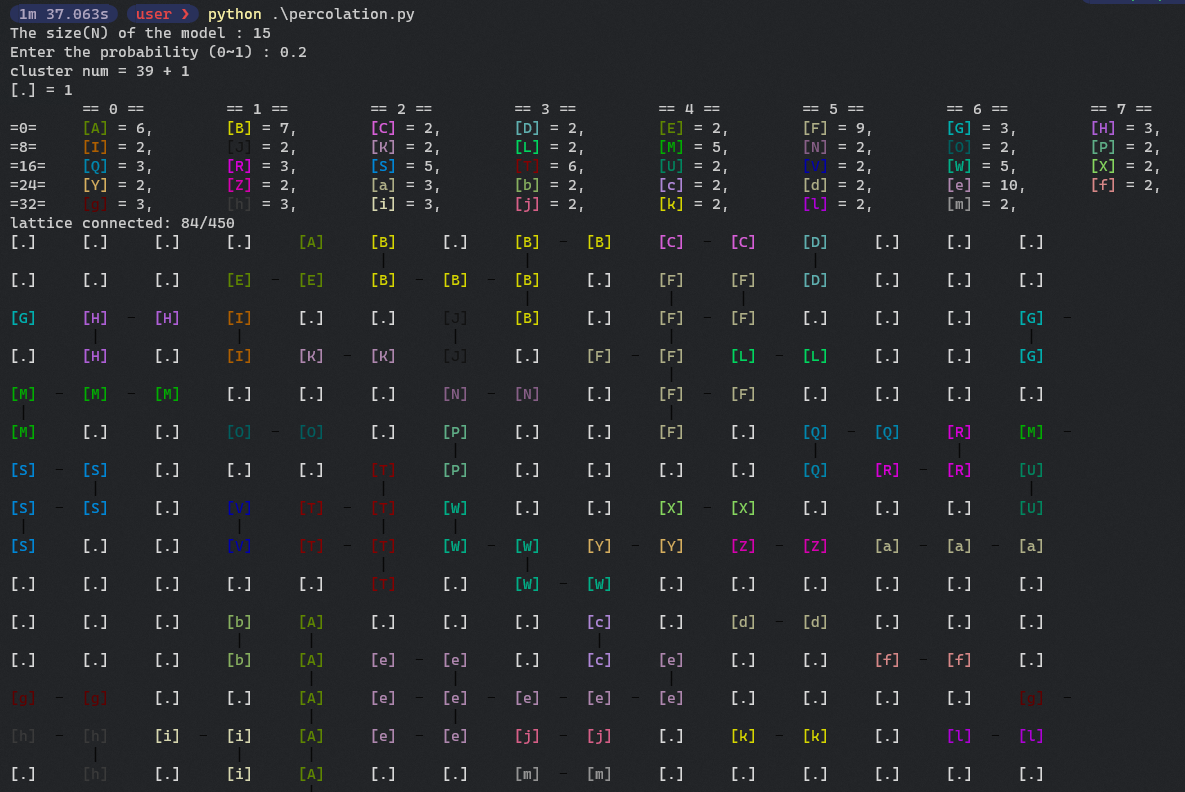
\includegraphics[width=1\linewidth]{percolation result with size = 15/size_15_prob_0.2.png}
     \caption{prob = 0.2}\label{prob = 0.2}
   \end{minipage}\hfill
   \begin{minipage}{0.48\textwidth}
     \centering
     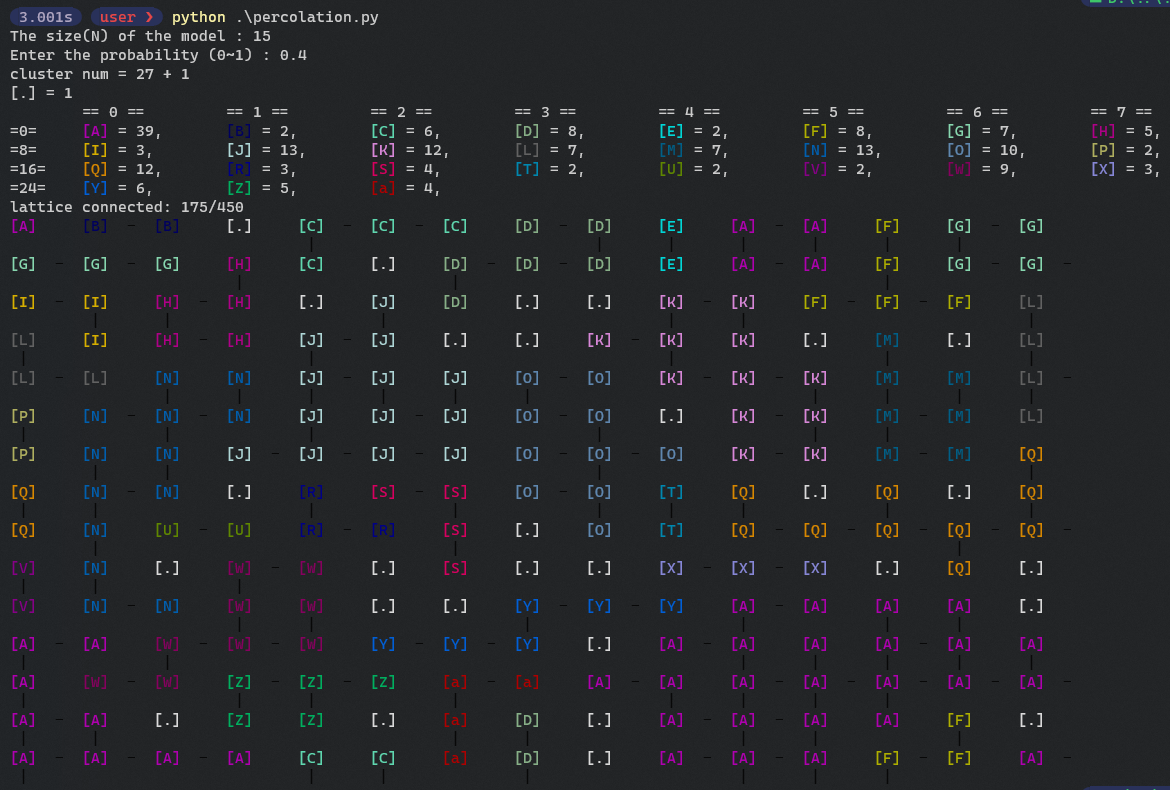
\includegraphics[width=1\linewidth]{percolation result with size = 15/size_15_prob_0.4.png}
     \caption{prob = 0.4}\label{prob = 0.4}
   \end{minipage}
\end{figure}


when the prob is 0.45, the largest clusters often connected more than 80 nodes, 

\begin{figure}[h]
\centering
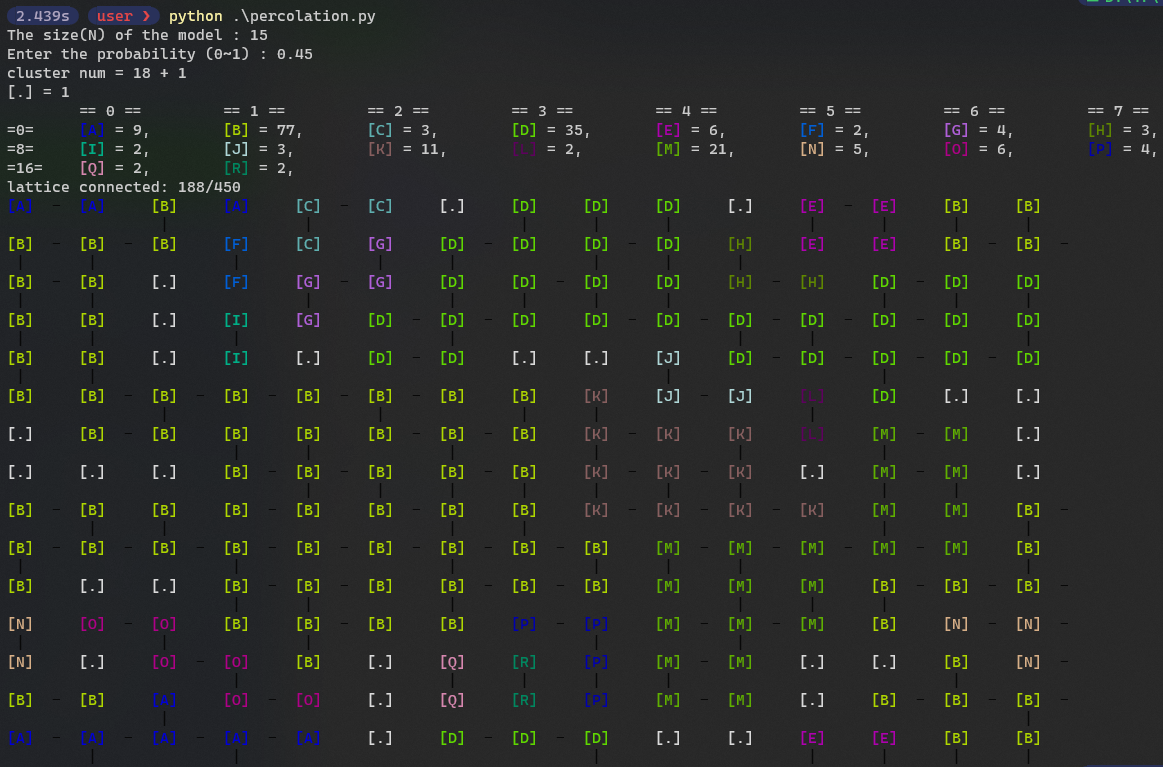
\includegraphics[width=0.465\linewidth]{percolation result with size = 15/size_15_prob_0.45.png}
\caption{\label{fig:DFS}prob = 0.45}
\end{figure}

\newpage

when the prob is over 0.45 the number of clusters decrease rapidly when the prob is increase until the 0.6.

\begin{figure}[h]
   \begin{minipage}{0.48\textwidth}
     \centering
     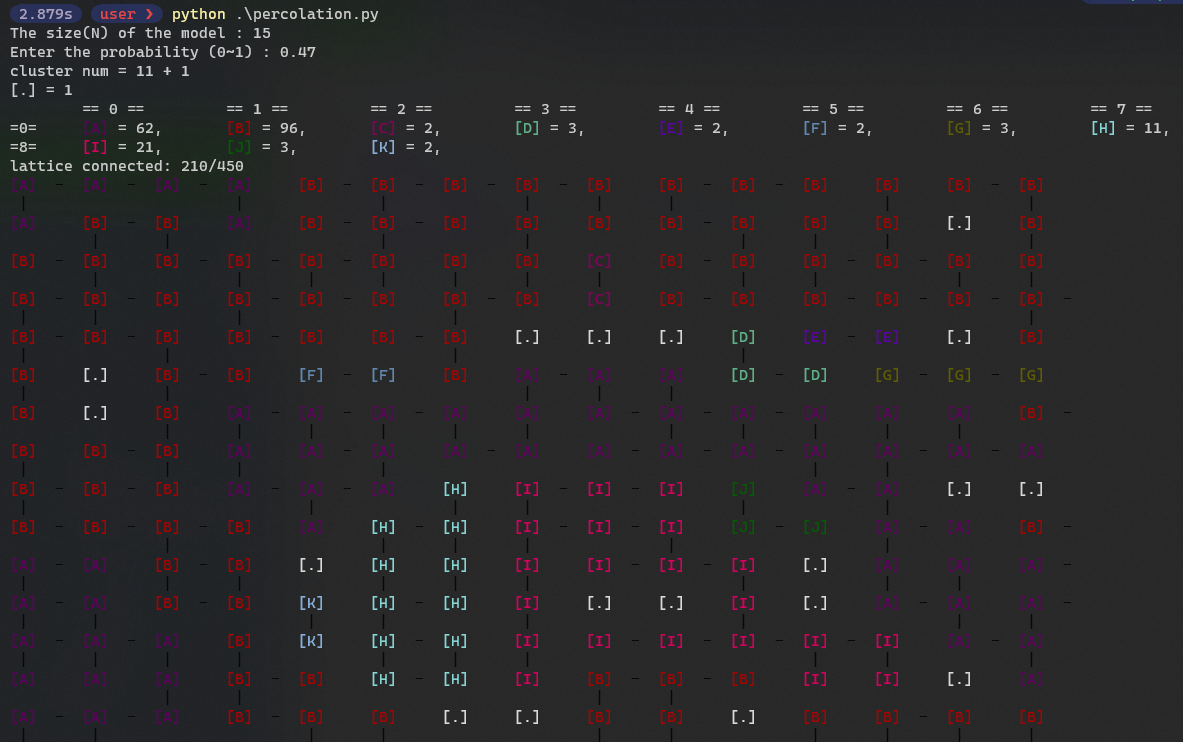
\includegraphics[width=1\linewidth]{percolation result with size = 15/size_15_prob_0.47.png}
     \caption{prob = 0.47}\label{prob = 0.47}
   \end{minipage}\hfill
   \begin{minipage}{0.48\textwidth}
     \centering
     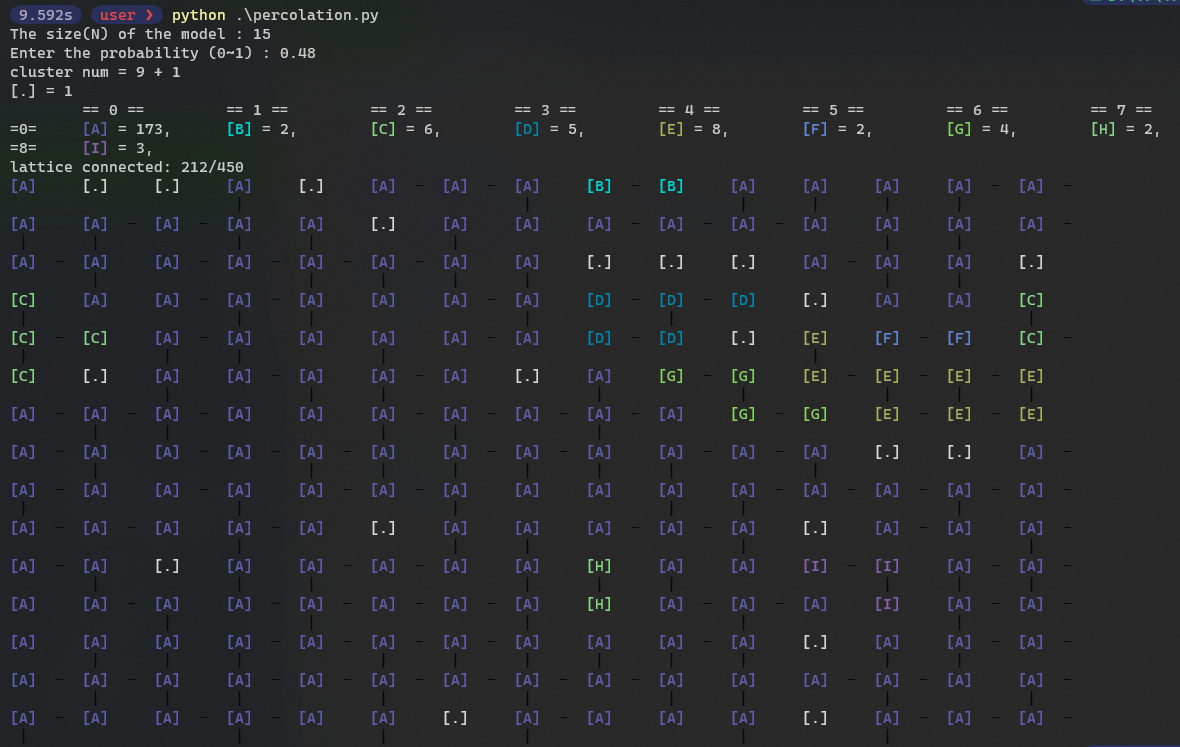
\includegraphics[width=1\linewidth]{percolation result with size = 15/size_15_prob_0.48.png}
     \caption{prob = 0.48}\label{prob = 0.48}
   \end{minipage}
\end{figure}

when the prob is over 0.55, the number of cluster is usually under 10, and most of the time there 

\begin{figure}[h]
   \begin{minipage}{0.48\textwidth}
     \centering
     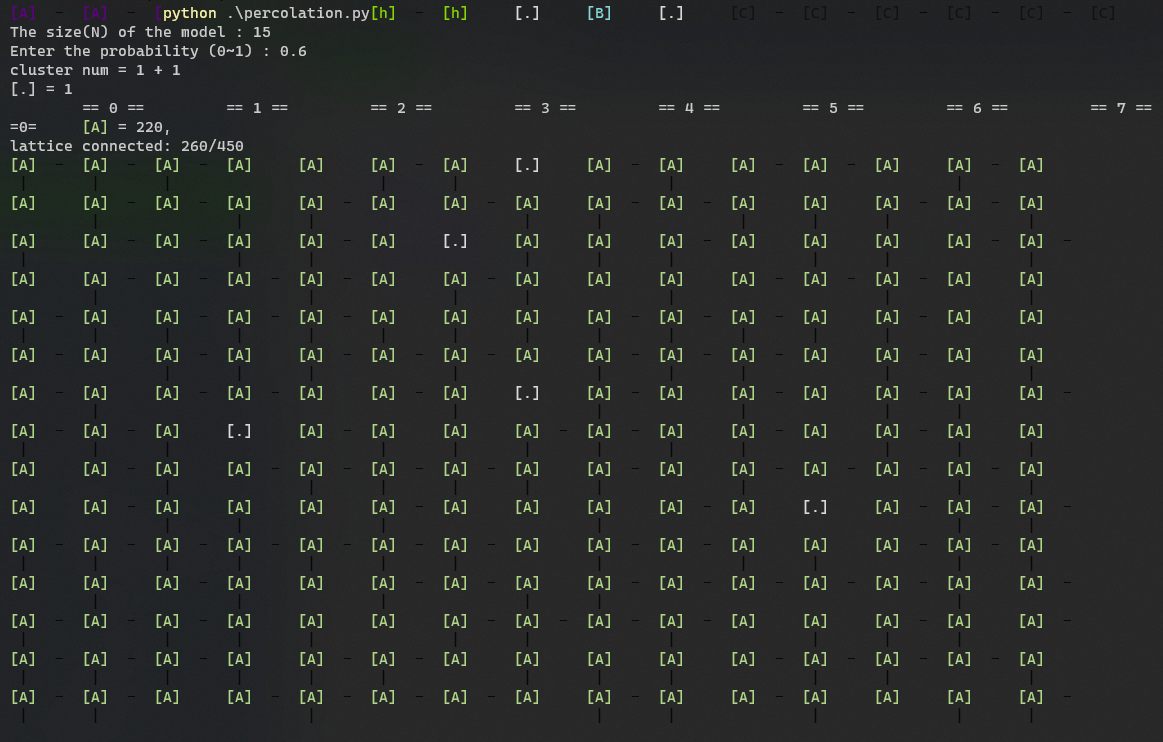
\includegraphics[width=1\linewidth]{percolation result with size = 15/size_15_prob_0.6.png}
     \caption{prob = 0.6}\label{prob = 0.6}
   \end{minipage}\hfill
   \begin{minipage}{0.48\textwidth}
     \centering
     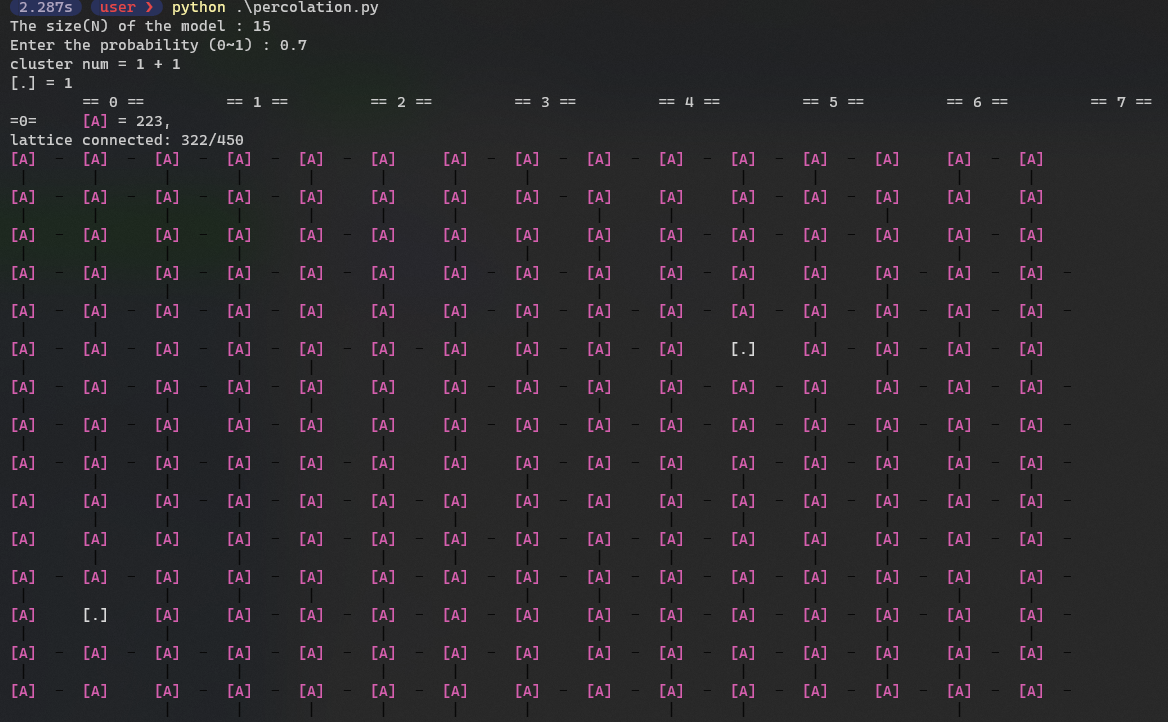
\includegraphics[width=1\linewidth]{percolation result with size = 15/size_15_prob_0.7.png}
     \caption{prob = 0.7}\label{prob = 0.7}
   \end{minipage}
\end{figure}

\section{Result}

In summary, after testing several time of the percolation the critical value of the probability is 0.45 when the model size is 15. Probability under critical number, there will be many clusters in the map; however, when the probability is over critical value, there will be only one or two large cluster that cover the whole map. The critical value will also increase to 0.5 if the model size is bigger than 15.

\end{document}